\documentclass[10pt,a4paper,twocolumn]{article}

\usepackage[margin=0.75in]{geometry}
\usepackage[T1]{fontenc}
\usepackage[utf8]{inputenc}
\usepackage{lmodern}
\usepackage{graphicx}
\usepackage{booktabs}
\usepackage{hyperref}
\usepackage{float}
\usepackage{array}
\usepackage{longtable}
\usepackage{setspace}

\hypersetup{
    colorlinks=true,
    linkcolor=black,
    citecolor=black,
    urlcolor=blue
}

\title{Language Identification in Very Short Texts:\\
The Effect of Length and Noise}
\author{Andrei-Cosmin Achim\\
Transilvania University of Brasov\\
\texttt{cosmin.achim@student.unitbv.ro}}
\date{}

\begin{document}

\maketitle
\thispagestyle{plain}

\begin{abstract}
Language identification is a standard preprocessing step in multilingual natural language processing pipelines, but the problem remains difficult when the input is extremely short and noisy. In this paper, I study language identification for short texts in five languages: English, Romanian, French, German, and Spanish. The experiments are designed around controlled text lengths of 3, 5, and 10 words, and around three input conditions: clean text, text without diacritics, and text containing a single synthetic typo. I compare three practical baselines: TF-IDF with Logistic Regression, character n-grams with Linear SVM, and fastText. The results show three consistent patterns. First, performance drops substantially at 3 words for all models. Second, character-based and subword-aware methods are markedly more robust to noise than the word-based baseline. Third, fastText and the character n-gram SVM offer the best trade-off between robustness and speed, while TF-IDF with Logistic Regression remains the fastest at inference time. The study provides a reproducible benchmark and a compact experimental setup that highlights the importance of evaluation conditions in short-text language identification.
\end{abstract}

\section{Introduction}

Language identification (LID) is the task of determining the language of a text segment. It is often treated as a solved problem for standard documents, but this impression becomes misleading once the input is very short, informal, or noisy. In practical applications such as comments, titles, chat messages, search queries, and user-generated snippets, the available text may contain only a few words and may also lack diacritics or include spelling mistakes. Under these conditions, many standard assumptions behind document-level language identification become weaker.

This topic is practically relevant for multilingual search, moderation pipelines, translation routing, and analytics systems. In all these settings, a wrong language prediction at the first stage can propagate errors to later components. For Romanian, French, German, Spanish, and English, the problem is especially interesting because these languages differ in their use of diacritics and in their degree of lexical overlap. Romanian and French are more visibly affected by diacritics, while English and German exhibit different character patterns and word formation behavior. More broadly, language identification belongs to the standard preprocessing toolkit of natural language processing systems, which makes the task relevant beyond this specific benchmark setting \cite{jurafsky2025slp}.

The motivation for this paper comes from a gap that is repeatedly noted in the literature. Existing work confirms that short-text LID remains difficult, that many evaluations are conducted on longer inputs, and that some high-performing approaches rely on metadata or user-specific information instead of text alone \cite{jauhiainen2019survey,balazevic2016shortsocial,duvenhage2019short}. For a compact and practically useful benchmark, it is important to isolate the text itself and test it under controlled degradations.

In this paper, I ask the following questions:

\begin{enumerate}
    \item How much does performance decrease when text length is reduced from 10 words to 5 and then to 3 words?
    \item How much do missing diacritics and minor spelling errors affect each model?
    \item What trade-off appears between predictive performance and inference speed?
\end{enumerate}

To answer these questions, I build a controlled benchmark over five languages and compare three baselines: TF-IDF with Logistic Regression, character n-grams with Linear SVM, and fastText \cite{joulin2017fasttext}. The rest of the paper is structured as follows. Section~\ref{sec:related} reviews relevant literature and positions the present work. Section~\ref{sec:method} describes the dataset, preprocessing, models, and evaluation design. Section~\ref{sec:results} presents the experimental findings and discusses their implications. Section~\ref{sec:conclusion} concludes the paper and highlights limitations and future work.

\section{Related Work and Critical Literature Review}
\label{sec:related}

Jauhiainen et al.\ provide a broad survey of automatic language identification and show that the task has a long history, many methodological variants, and a strong dependence on evaluation setup \cite{jauhiainen2019survey}. The survey is especially important for this paper because it emphasizes that results obtained on longer documents do not directly transfer to short texts. It also highlights that lexicon-based methods can suffer from unrealistic evaluation settings when the lexicon is constructed using information from both train and test data. This observation is directly relevant for designing a fair experiment.

Balazevic et al.\ study language detection for short social media messages and show that short texts introduce additional challenges such as abbreviations, spelling variation, and informal writing \cite{balazevic2016shortsocial}. Their work is useful because it focuses on short inputs instead of standard documents. At the same time, one of its strongest ideas is the incorporation of personalized user-specific information. This can indeed improve results in social media settings, but such metadata is not always available and reduces the generality of the method. For this reason, the present work restricts itself to text-only classification.

Duvenhage investigates short-text language identification for under-resourced languages and argues that evaluation methodology is still a major issue in the field \cite{duvenhage2019short}. This paper is valuable because it combines short inputs with difficult language distinctions and discusses the danger of comparing methods across incompatible experimental conditions. The work also reinforces the broader conclusion that short-text LID remains an open research problem.

From the modeling perspective, fastText is a strong practical baseline because it combines word and subword information while remaining computationally efficient \cite{joulin2017fasttext}. Character n-gram models have a long tradition in text categorization and language identification, going back to classic work such as Cavnar and Trenkle \cite{cavnar1994ngram}; later practical systems and software implementations also confirmed the usefulness of n-gram profiles for language-related categorization tasks \cite{hornik2013textcat}. Character n-gram models have also been repeatedly shown to be competitive in language identification because they capture orthographic patterns that are robust to short contexts and spelling variation \cite{jauhiainen2019survey}. By contrast, word-based TF-IDF baselines are often fast and simple but can be more brittle when the text is extremely short or noisy.

The main methodological gap that remains insufficiently addressed in the literature is the need for a simple, text-only, controlled benchmark that jointly varies input length and realistic noise. Many papers either evaluate on longer texts, focus on different language sets, rely on metadata, or make comparisons that are difficult to align across datasets. The contribution of the present work is modest but useful: it defines a reproducible benchmark over five European languages, uses fixed text lengths of 3, 5, and 10 words, injects two noise types with clear practical relevance, and compares three accessible baselines under the same protocol.

\section{Methodology and Case Study}
\label{sec:method}

\subsection{Research Design}

The study evaluates language identification under controlled short-text conditions. The target languages are English (EN), Romanian (RO), French (FR), German (DE), and Spanish (ES). The experiment is based on three text lengths and three noise conditions, resulting in nine evaluation settings:

\begin{itemize}
    \item text lengths: 3, 5, and 10 words;
    \item noise conditions: clean, no\_diacritics, and typo.
\end{itemize}

The methodology is intentionally simple. Models are trained only on clean texts and are then evaluated on both clean and degraded inputs. This makes robustness easier to interpret because performance drops cannot be attributed to different training conditions.

\subsection{Dataset and Preprocessing}

The dataset used in the final experiments is \texttt{agentlans/high-quality-multilingual-sentences}, accessed through Hugging Face.\footnote{\url{https://huggingface.co/datasets/agentlans/high-quality-multilingual-sentences}} From the available language-specific configurations, only EN, RO, FR, DE, and ES are retained. For each language, 2000 examples are sampled after cleaning and filtering.

The cleaning stage includes:

\begin{itemize}
    \item retaining only the five target languages;
    \item removing empty rows and duplicate text-label pairs;
    \item normalizing whitespace;
    \item keeping only texts with at least 10 words.
\end{itemize}

The dataset is then split in a stratified manner into 80\% train, 10\% validation, and 10\% test. This results in the same class balance for each split:

\begin{itemize}
    \item 1600 train examples per language;
    \item 200 validation examples per language;
    \item 200 test examples per language.
\end{itemize}

\subsection{Controlled Shortening and Noise Injection}

From each retained sentence, three short-text variants are generated by keeping the first 3, 5, and 10 words. This creates a controlled comparison across lengths while preserving the same source sentence identity.

Three surface conditions are then constructed:

\begin{itemize}
    \item \textbf{clean}: original shortened text;
    \item \textbf{no\_diacritics}: diacritics removed with a deterministic normalization function;
    \item \textbf{typo}: one deterministic synthetic character substitution per text.
\end{itemize}

The typo generation is seeded in a reproducible way using the source identifier and the length bucket, so the same experiment always produces the same noisy text.

\subsection{Models}

Three baselines are evaluated:

\begin{enumerate}
    \item \textbf{TF-IDF + Logistic Regression}: a word-based baseline using unigram and bigram TF-IDF features;
    \item \textbf{Character n-grams + Linear SVM}: a stronger LID baseline using character TF-IDF with 3--5-gram features;
    \item \textbf{fastText}: a supervised classifier trained with subword information and word n-grams.
\end{enumerate}

The choice of models is motivated by practicality and interpretability. Logistic Regression serves as a simple lexical baseline, the character n-gram SVM represents a traditional strong LID approach, and fastText serves as a fast industrial-style baseline.

\subsection{Evaluation Protocol}

Each model is trained separately for each length bucket on the \texttt{train} split with \texttt{clean} texts only. Evaluation is then performed on the \texttt{val} and \texttt{test} splits for the same length bucket under all three conditions.

The main metrics are:

\begin{itemize}
    \item accuracy;
    \item macro-F1;
    \item inference throughput in examples per second.
\end{itemize}

\section{Experimental Results and Discussion}
\label{sec:results}

\subsection{Overall Results}

Table~\ref{tab:overall} summarizes mean test performance across all conditions.

\begin{table}[H]
\centering
\caption{Average test performance across all length and noise conditions.}
\label{tab:overall}
\begin{tabular}{lccc}
\toprule
Model & Accuracy & Macro-F1 & Examples/sec \\
\midrule
char\_svm & 0.9601 & 0.9601 & 38644.8 \\
fasttext & 0.9553 & 0.9554 & 99264.1 \\
tfidf\_lr & 0.9058 & 0.9083 & 224343.9 \\
\bottomrule
\end{tabular}
\end{table}

These averages already suggest the main trade-off. The character n-gram SVM is the strongest overall model, fastText is very close while being substantially faster, and TF-IDF with Logistic Regression is by far the fastest but clearly weaker in accuracy.

\begin{figure}[H]
\centering
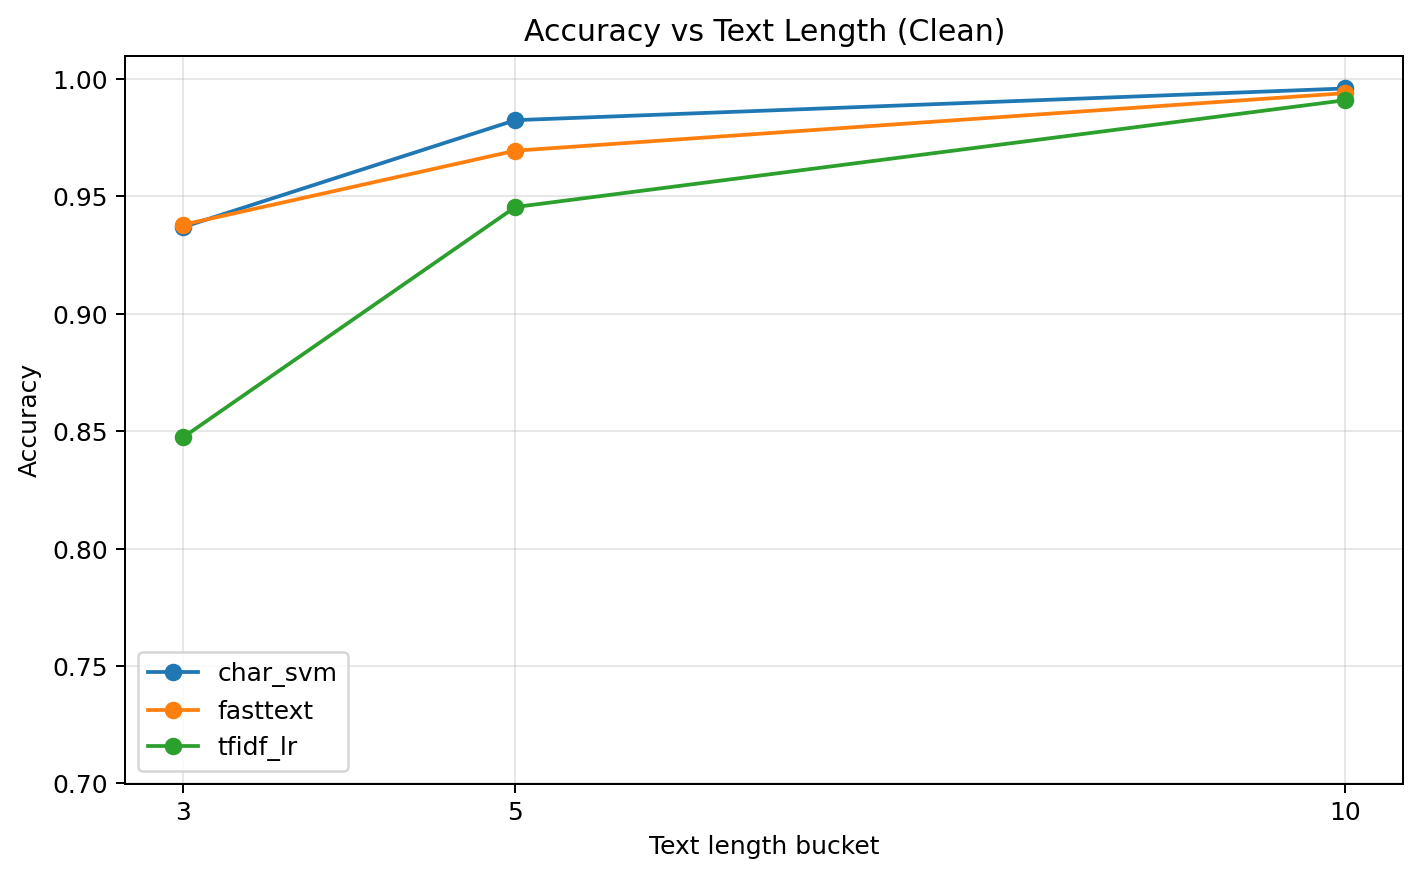
\includegraphics[width=\columnwidth]{../results/plots/accuracy_by_length_clean.png}
\caption{Average accuracy on clean text as a function of text length.}
\label{fig:accuracy_length}
\end{figure}

\subsection{Effect of Text Length}

The strongest pattern in the experiments is the sharp improvement that appears when moving from 3 words to 5 words and then to 10 words. For example, on the clean test condition:

\begin{itemize}
    \item \textbf{3 words}: fastText reaches 0.934, char\_svm 0.927, and tfidf\_lr 0.846;
    \item \textbf{5 words}: char\_svm reaches 0.982, fastText 0.966, and tfidf\_lr 0.944;
    \item \textbf{10 words}: char\_svm reaches 0.994, fastText 0.991, and tfidf\_lr 0.990.
\end{itemize}

This confirms the central hypothesis of the project: short-text LID becomes significantly harder when the available context drops to only a few words. With 10 words, all three models are highly competitive. With 3 words, the gap between robust models and the lexical baseline becomes much wider.

\subsection{Effect of Noise}

\begin{figure}[H]
\centering
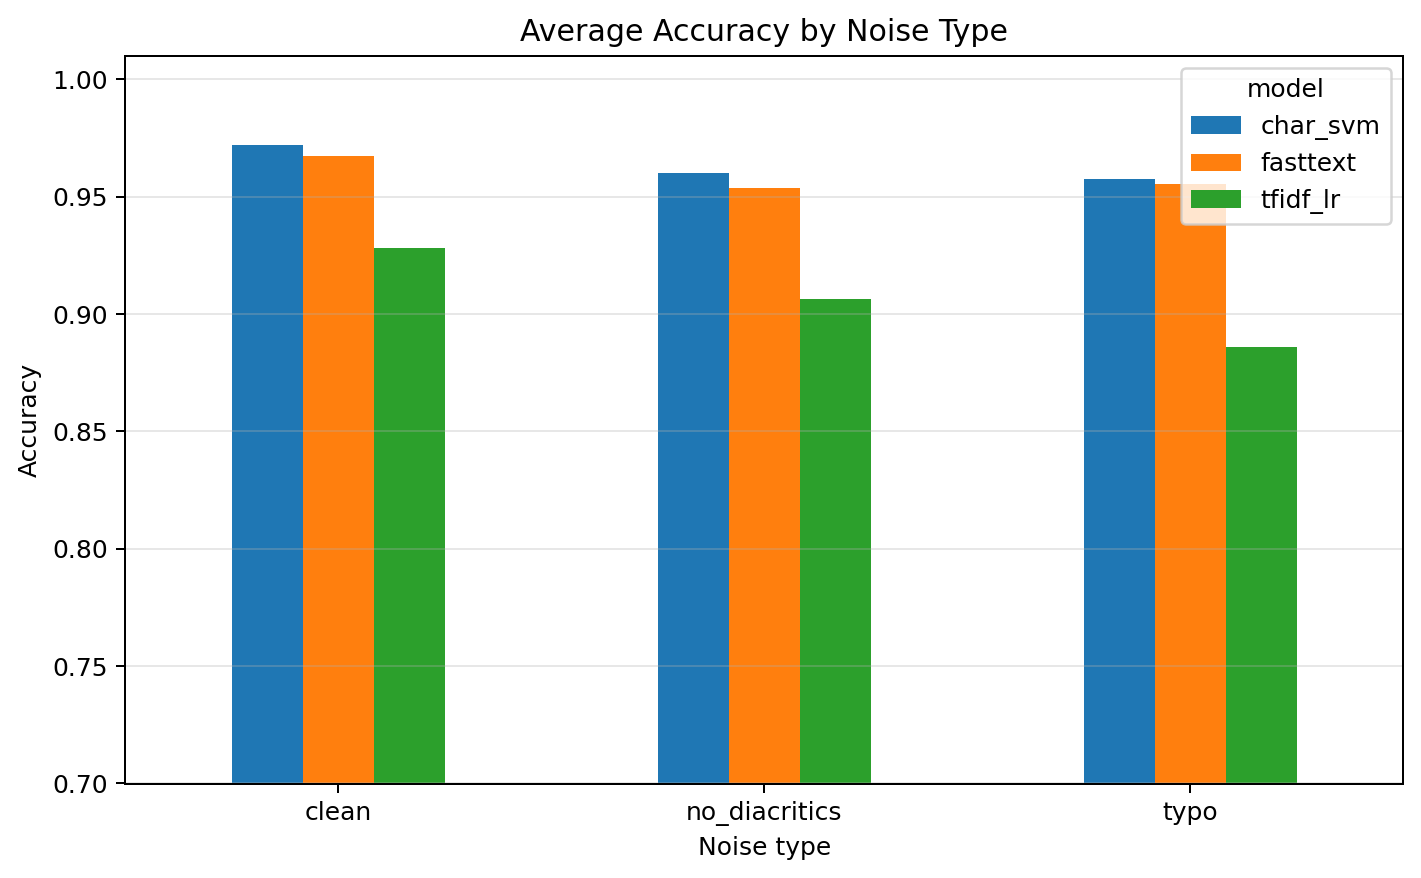
\includegraphics[width=\columnwidth]{../results/plots/accuracy_by_noise.png}
\caption{Average accuracy by noise condition across models.}
\label{fig:accuracy_noise}
\end{figure}

Noise has the strongest impact at 3 words. In that setting:

\begin{itemize}
    \item char\_svm drops from 0.927 on clean text to 0.899 without diacritics and 0.908 with a typo;
    \item fastText drops from 0.934 to 0.911 and 0.909, respectively;
    \item tfidf\_lr drops from 0.846 to 0.818 and 0.758.
\end{itemize}

The typo condition is especially harmful for the word-based baseline because a one-character perturbation can destroy a token match. By contrast, character n-grams and fastText retain subword signals and are therefore more robust. At 10 words, the degradation becomes much smaller because the models can compensate using the remaining context.

\subsection{Per-Language Analysis}

Per-language test averages also reveal that the languages are not equally difficult. Averaged over models and conditions, the mean accuracies are:

\begin{itemize}
    \item FR: 0.9196
    \item EN: 0.9365
    \item ES: 0.9365
    \item RO: 0.9515
    \item DE: 0.9580
\end{itemize}

In this setup, French is the most difficult language and German the easiest. This is an empirical observation rather than a universal claim. A plausible explanation is that French suffers more under the loss of diacritics and shares many short lexical patterns with other Romance languages in the benchmark, especially Spanish and Romanian. German, on the other hand, may benefit from distinctive orthographic patterns captured well by character n-grams and subword models.

\subsection{Error Analysis on the Hardest Scenario}

To better understand model behavior beyond aggregate metrics, I also examined the hardest realistic condition in the benchmark: the test split with 3-word texts and one synthetic typo. Under this setting, fastText was the best-performing model, with an accuracy of 0.909. Figure~\ref{fig:confusion_hardest} shows the normalized confusion matrix for this case.

\begin{figure}[H]
\centering
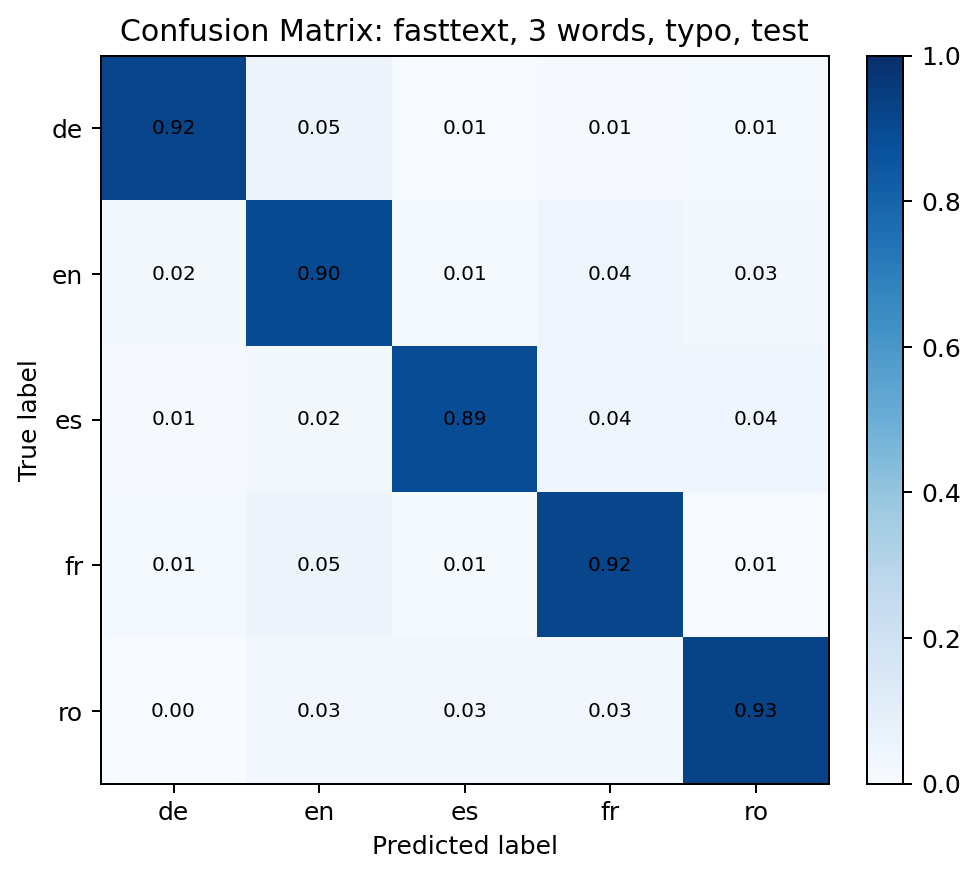
\includegraphics[width=\columnwidth]{../results/error_analysis/fasttext_len3_typo_test_confusion_matrix.png}
\caption{Normalized confusion matrix for fastText on the hardest condition: 3-word texts with one typo on the test split.}
\label{fig:confusion_hardest}
\end{figure}

The dominant confusions are linguistically plausible. German is sometimes predicted as English (5\%), French is also confused with English (5\%), and English is confused with French (4.5\%). Spanish is split mainly between French and Romanian (4\% each), while Romanian is occasionally confused with English, Spanish, and French (2.5\% each). These patterns suggest that once the available context is reduced to only three noisy words, the classification problem becomes less about full lexical evidence and more about short orthographic fragments, shared Romance vocabulary, and incomplete subword cues. This analysis supports the broader conclusion that global averages alone are not sufficient: the error structure itself is informative and reveals where short-text language identification remains fragile.

\subsection{Interpretation}

\begin{figure}[H]
\centering
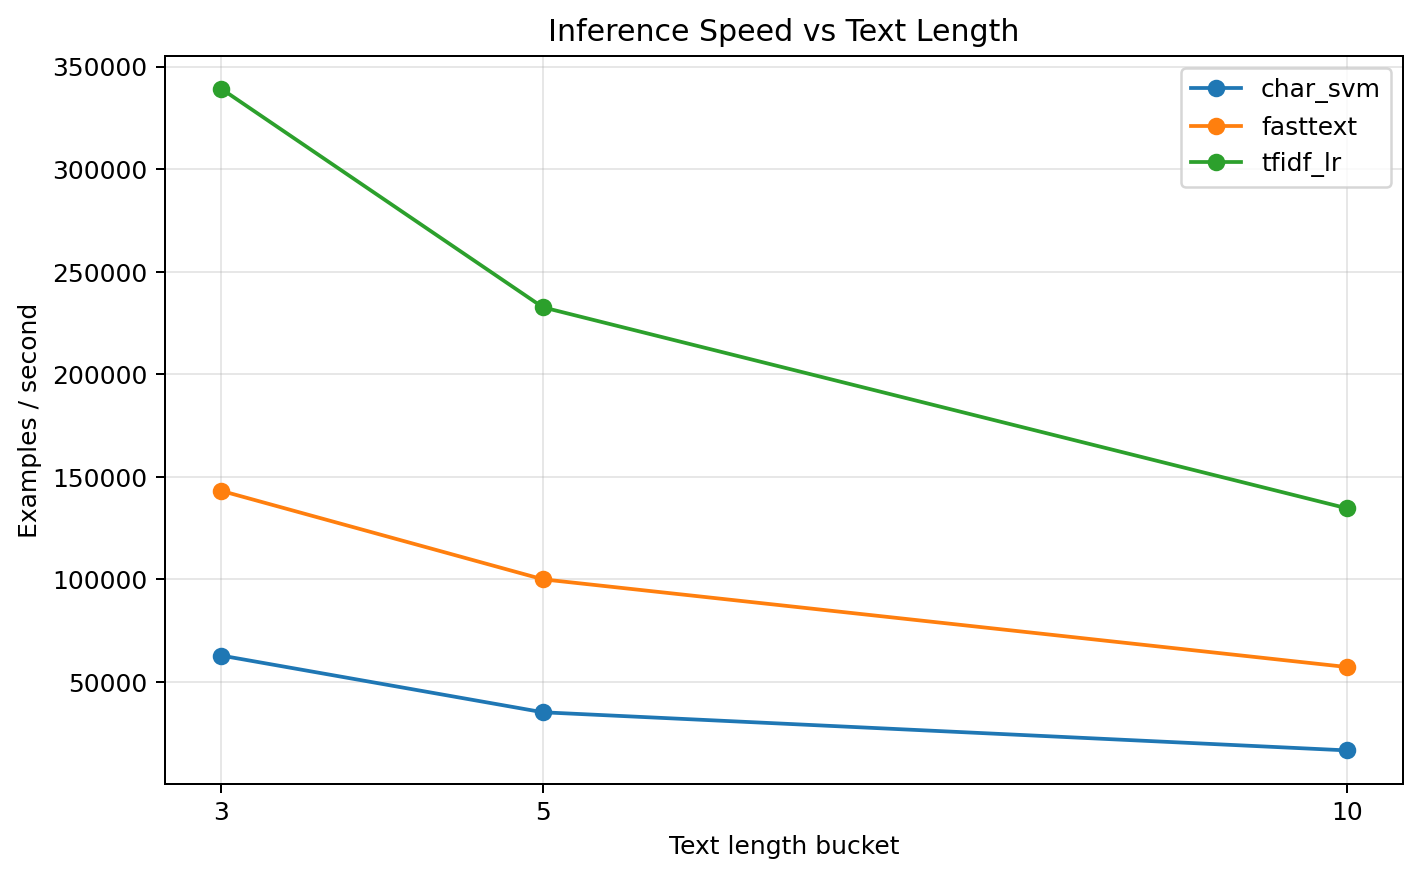
\includegraphics[width=\columnwidth]{../results/plots/speed_by_length.png}
\caption{Inference speed as a function of text length.}
\label{fig:speed_length}
\end{figure}

The results lead to three main conclusions.

First, short-text language identification should not be evaluated only on clean, document-length inputs. A model that performs very well on 10-word snippets can still behave much worse at 3 words.

Second, text representation matters more than classifier sophistication in this setup. The difference between the word-based TF-IDF baseline and the character/subword-based models is substantial under the hardest conditions.

Third, fastText is particularly attractive when a strong performance-speed trade-off is needed. It is not the absolute best model on average, but it dominates the 3-word clean and noisy conditions in this experiment and remains much faster than the SVM.

\section{Conclusion}
\label{sec:conclusion}

This paper presented a controlled study of short-text language identification under realistic degradation conditions. The benchmark covered five languages, three short-text lengths, and three noise conditions, and compared three practical baselines.

The experiments showed that:

\begin{itemize}
    \item performance decreases sharply when text length is reduced to 3 words;
    \item missing diacritics and spelling noise are especially harmful in the shortest setting;
    \item character-based and subword-aware approaches are clearly more robust than a lexical TF-IDF baseline;
    \item char\_svm is the strongest model overall, while fastText offers an excellent balance between robustness and speed.
\end{itemize}

The study also has limitations. The benchmark uses only five languages and one public dataset, and the shortening strategy retains the first $N$ words rather than sampling arbitrary spans. The typo model is intentionally simple and deterministic, which is good for reproducibility but does not fully capture natural user errors. Finally, no transformer-based multilingual model was evaluated in the current version.

Future work can extend the benchmark with additional language families, per-language confusion analysis, stronger noise models, and a multilingual transformer baseline. Even in its present form, however, the study provides a reproducible and practically meaningful comparison for language identification on very short noisy texts.

\bibliographystyle{plain}
\bibliography{references}

\end{document}
